%% Epilogue — 지루한 서비스
\frontchapter{지루한 서비스}{에필로그}
\chaptersubtitle{15주, 하나의 대화 모델, 아무 일도 일어나지 않았다는 조용한 승리}

\begin{calloutbox}{tbbblue}{tbbbluefill}
{\normalsize\bfseries\color{tbbblue}이 맺음말에 있는 것과 없는 것}\par\vspace{3pt}
이 맺음말에는 학습 목표도, 실습도, 연습문제도 없으며 시험에 나올 내용도 없다. 실제로 다녀온 여행을 다룬 박물관을 걷듯 읽으면 된다. 데모를 마친 뒤 커피 한 잔을 들고, 즐거운 속도로 천천히 둘러보자. 여기에는 여러분이 만든 서비스의 \textbf{일대기}, 직접 얻은 한 줄 문장을 모은 \textbf{기념품 진열장}, 이제 참석할 자격이 생긴 \textbf{저녁 만찬}, 이 책의 어떤 내용이 곧 만료되고 무엇이 10년 동안 보증되는지 적은 \textbf{보증서}, 아직 겪지 않았지만 언젠가는 찾아올 밤을 위한 짧은 \textbf{편지}가 들어 있다.
\end{calloutbox}

\vspace{4.0pt}

\namedsection{E.1}{한 서비스의 일대기}

이 서비스는 1주 차에 부끄러운 모습으로 태어났다. 완벽한 모델 실행에는 0.31초가 걸렸지만, 그 앞뒤를 \textbf{30초의 침묵과 빙글빙글 도는 커서}가 감쌌다. 사례 1-A의 진짜 주제는 버그 자체가 아니었다. 첫 요청에서 차가운 모델을 불러오고, 아무도 그리지 않은 대기열이 생긴 일이 전부가 아니었다. 핵심은 한 학기 내내 배운 끝에 두 줄로 내릴 수 있게 된 진단, 곧 \textit{어느 구간이 병목인가?}라는 질문이었다. 그 진단 속에는 더 큰 선언이 숨어 있었다. 학습된 모델과 작동하는 서비스는 서로 다른 결과물이며, 그 둘 사이에는 이 책의 모든 내용이 놓여 있다. 이 서비스의 첫 주는 여느 서비스와 같았다. 완벽한 두뇌는 있었지만 몸도, 예의도, 약속도 없었고 무엇에 얼마가 드는지도 몰랐다.

2주 차부터 5주 차까지는 몸을 만드는 시간이었다. 서비스는 \textbf{머신}을 얻었고, 곧 그 머신이 공손한 허구임을 배웠다. 하이퍼바이저 위의 손님일 뿐이며, GPU만은 패스스루가 허구의 틈으로 실리콘을 손대지 않고 건네기 때문에 실제였다. 빌린 것 가운데 가상화되지 않은 유일한 부분이 바로 돈을 내는 부분이다. 이어 \textbf{울타리와 계량기}를 얻었다. 네임스페이스는 자기 자신만 보게 했고, cgroup은 자기 몫만 먹게 했다. 그리고 처음 죽었다. \code{exit 137}, 커널의 작별 인사다. 이 책에서 영원히 외우라고 요구하는 유일한 계산이기도 하다(128 + signal 9). 다음에는 \textbf{운반할 수 있는 몸}을 얻었다. 계층으로 쌓고 다이제스트로 고정한 이미지 덕분에 "내 머신에서는 되는데"가 "어디서나 바이트 단위로 똑같은 내 머신 그 자체"로 바뀌었다. 마지막으로 \textbf{반사 작용}을 얻었다. 프로브는 트래픽을 통제하고, 재시작은 회의를 기다리지 않는다. 플릿 관리자는 사용자의 의도를 데이터베이스로, 현실을 고쳐야 할 버그로 취급한다. 5주 차가 되자 서비스는 자신의 죽음에서도 살아남을 수 있었다. 그러나 아직 \textit{신뢰할} 수는 없었다. 반사 작용은 행동하지만 설명하지 못한다. 그 빚은 14주 차까지 조용히 남아 있었다.

6주 차에는 \textbf{문}이 생겼다. 로드 밸런서, TLS, 키, 할당량으로 이루어진 문이었다. 이 문과 함께 강의에서 처음으로 진짜 상업적인 문장이 등장했다. \textit{curl에 답하는 컨테이너}와 \textit{누군가에게 요금을 청구할 수 있는 서비스}의 차이는 문이다. 문은 외부 세계가 거절을 표현하는 여러 어휘도 알려 주었다. 503과 504, 문장 중간에서 끊기는 스트림이 그것이다. 또한 자기 벽 바깥에 서서 안쪽을 점검하는 규율을 가르쳤다. 6주 차에는 편집증처럼 보였던 습관이 14주 차에는 호출 정책이 되었다.

7주 차는 사춘기였다. 서비스는 \textbf{약속하는 법}을 배웠다. 막연히 "빨라야 한다"가 아니라 형태가 있는 약속이었다. \textit{이 위치에서, 이 시간 구간 동안, 이 부하와 이 예산 아래에서 측정한 p99가 500ms 이하여야 한다.} 백분위수의 문법도 배웠다. 평균은 아무도 설명하지 못하고, 백분위수는 더할 수도 평균 낼 수도 없다. 이 규칙은 이후 히스토그램을 입고 두 번 더 돌아왔다. 서비스는 용돈, 즉 오류 예산도 받았다. 덕분에 신뢰성은 미덕을 겨루는 일이 아니라 장부를 관리하는 일이 되었다. 그러자 첫 청구서가 도착했다. 단순하게 구성한 플릿의 월 비용은 \textbf{4,762달러}였다. 이 숫자는 부모가 치켜뜬 눈썹처럼 5주 동안 강의 위에 걸려 있었다. 9주 차에는 군중이 몰려왔다. 서비스는 대부분의 폭풍이 스스로 만든 것임을 배웠다. 재시도 폭풍은 이 책에서 피해자가 직접 조직하는 유일한 기상 현상이다. 그리고 일찍, 싸게 거절하는 법을 익혔다. \textit{거절이 곧 제품이다.} 10주 차에는 절차를 갖춰 다이어트를 시작했다. 비용을 절반으로 줄이는 INT8은 측정 \textit{전에} 허용 오차를 적어 둔 관문을 통과해야만 허용되었다. 판정 관문 없는 손실 최적화는 규모만 커진 희망 사항일 뿐이기 때문이다. 청구서는 \textbf{2,381달러}로 내려갔다.

11주 차에 서비스는 \textbf{말하는 법}을 배웠고, 말하기는 서비스의 물리 법칙을 바꾸었다. 하나였던 지연 시간은 두 개의 시계가 되었다. 첫 단어를 기다리는 시간과 그 뒤 단어가 나오는 속도다. 메모리는 부동산이 되었다. KV 캐시는 토큰당 112KB, 긴 대화 하나에는 448MiB가 필요했다. 테이블의 좌석은 메가바이트 단위로 값을 매겼고 연속 배칭으로 채웠다. 위대한 할당 기법인 PagedAttention은 malloc의 오래된 비극, 즉 최댓값만큼 예약하고 차이는 버리는 문제를 1962년 운영체제가 해결한 방식으로 고쳤다. 페이지 테이블이다. 스트리밍에 맞춰 SLO를 공개적으로, 계산을 보이며 다시 협상했다. 12주 차에는 \textbf{호흡하는 법}을 배웠다. 하루의 계단을 따라 레플리카가 움직였다. 파드는 파도를 쫓고, 노드는 예보를 따랐다. 콜드 스타트의 150초도 숨기지 않고 비용에 넣었다. 새뮤얼 인설이 전기를 팔던 방식으로 용량을 샀다. 기본 부하는 약정 용량으로, 피크는 스팟으로 감당하고 골짜기에는 유용한 일을 찾아 넣었다. 청구서는 \textbf{1,513달러}, 이어 \textbf{877달러}로 줄었다. 그리고 강의에서 가장 조용한 교훈이 남았다. \textit{자체 구축 대 외부 도입은 구호였던 적이 없다. 언제나 부하율의 문제였다.}

13주 차에는 \textbf{소란 없이 바꾸는 법}을 배웠다. 금요일 배포에서 완벽한 모델이 홀로 이동한 설정 파일 하나 때문에 망가졌다. 이 사건은 레지스트리, 파이프라인, 카나리를 낳았다. 릴리스는 증거를 붙인 다이제스트 \textit{세 개}의 묶음이 되었고, 파이프라인의 빨간 실행 결과는 일어나지 않은 금요일이라는 제품이 되었다. 홀데인의 새는 자동 후퇴 반사 작용을 지닌 카나리로 다시 태어났다. 배포는 엔지니어링에서 가장 지루한 문장으로 바뀌었다. \textit{자동화되고, 버전이 있으며, 점진적이고, 되돌릴 수 있다.} 14주 차에는 반사 작용에 없던 세 가지를 더해 신경계를 완성했다. \textbf{기억}은 새벽 2시의 두뇌가 질문하는 순서대로 배치한 네 줄의 대시보드였다. \textbf{주의}는 감이 아니라 소진율을 보고, 그것도 드물게 울리는 호출이었다. 경보 피로에는 실제 희생자가 있기 때문이다. \textbf{예지}는 매주 드리프트를 지켜보는 일이었다. 카나리는 절벽을 잡지만 세상은 비탈을 더 좋아한다. 첫 실제 장애는 12주 차에 예고한 바로 그 수수께끼, 같은 GPU를 쓰는 이웃 때문에 일어났다. 장애는 20분 만에 끝났고, 세 개의 조치 항목과 비난 0건을 남겼다. 마지막 청구 금액은 \textbf{정확히 900달러}였다. 마지막 23달러는 나머지 모든 부분을 감시하는 부분의 비용이었다.

그리고 15주 차, 서비스는 낯선 사람들 앞에 서서 시연되었다. 모든 것이 설계대로였다면 데모는, 자랑스럽게 말하자, \textbf{지루했다.} 트래픽은 키가 달린 문을 통과했고, 답은 숫자로 적은 약속 안에서 나왔다. 청구서는 스스로 선택한 금액으로 끝났고, 프로젝터 한쪽에서는 대시보드가 잔잔히 숨 쉬었다. 운영에서 지루함은 흥분이 없다는 뜻이 아니다. 관문과 리허설, 오후 2시에 미리 그린 그래프로 흥분의 값을 \textit{선불로 치렀다}는 뜻이다. 이 서비스의 일대기는 훌륭한 모든 인프라의 일대기와 같은 방식으로 끝난다. 공개된 자리에서, 의도한 대로, 아무 일도 일어나지 않는다.

\begin{tbbfigure}
  \adjustbox{max width=0.94\linewidth,max totalheight=0.46\textheight}{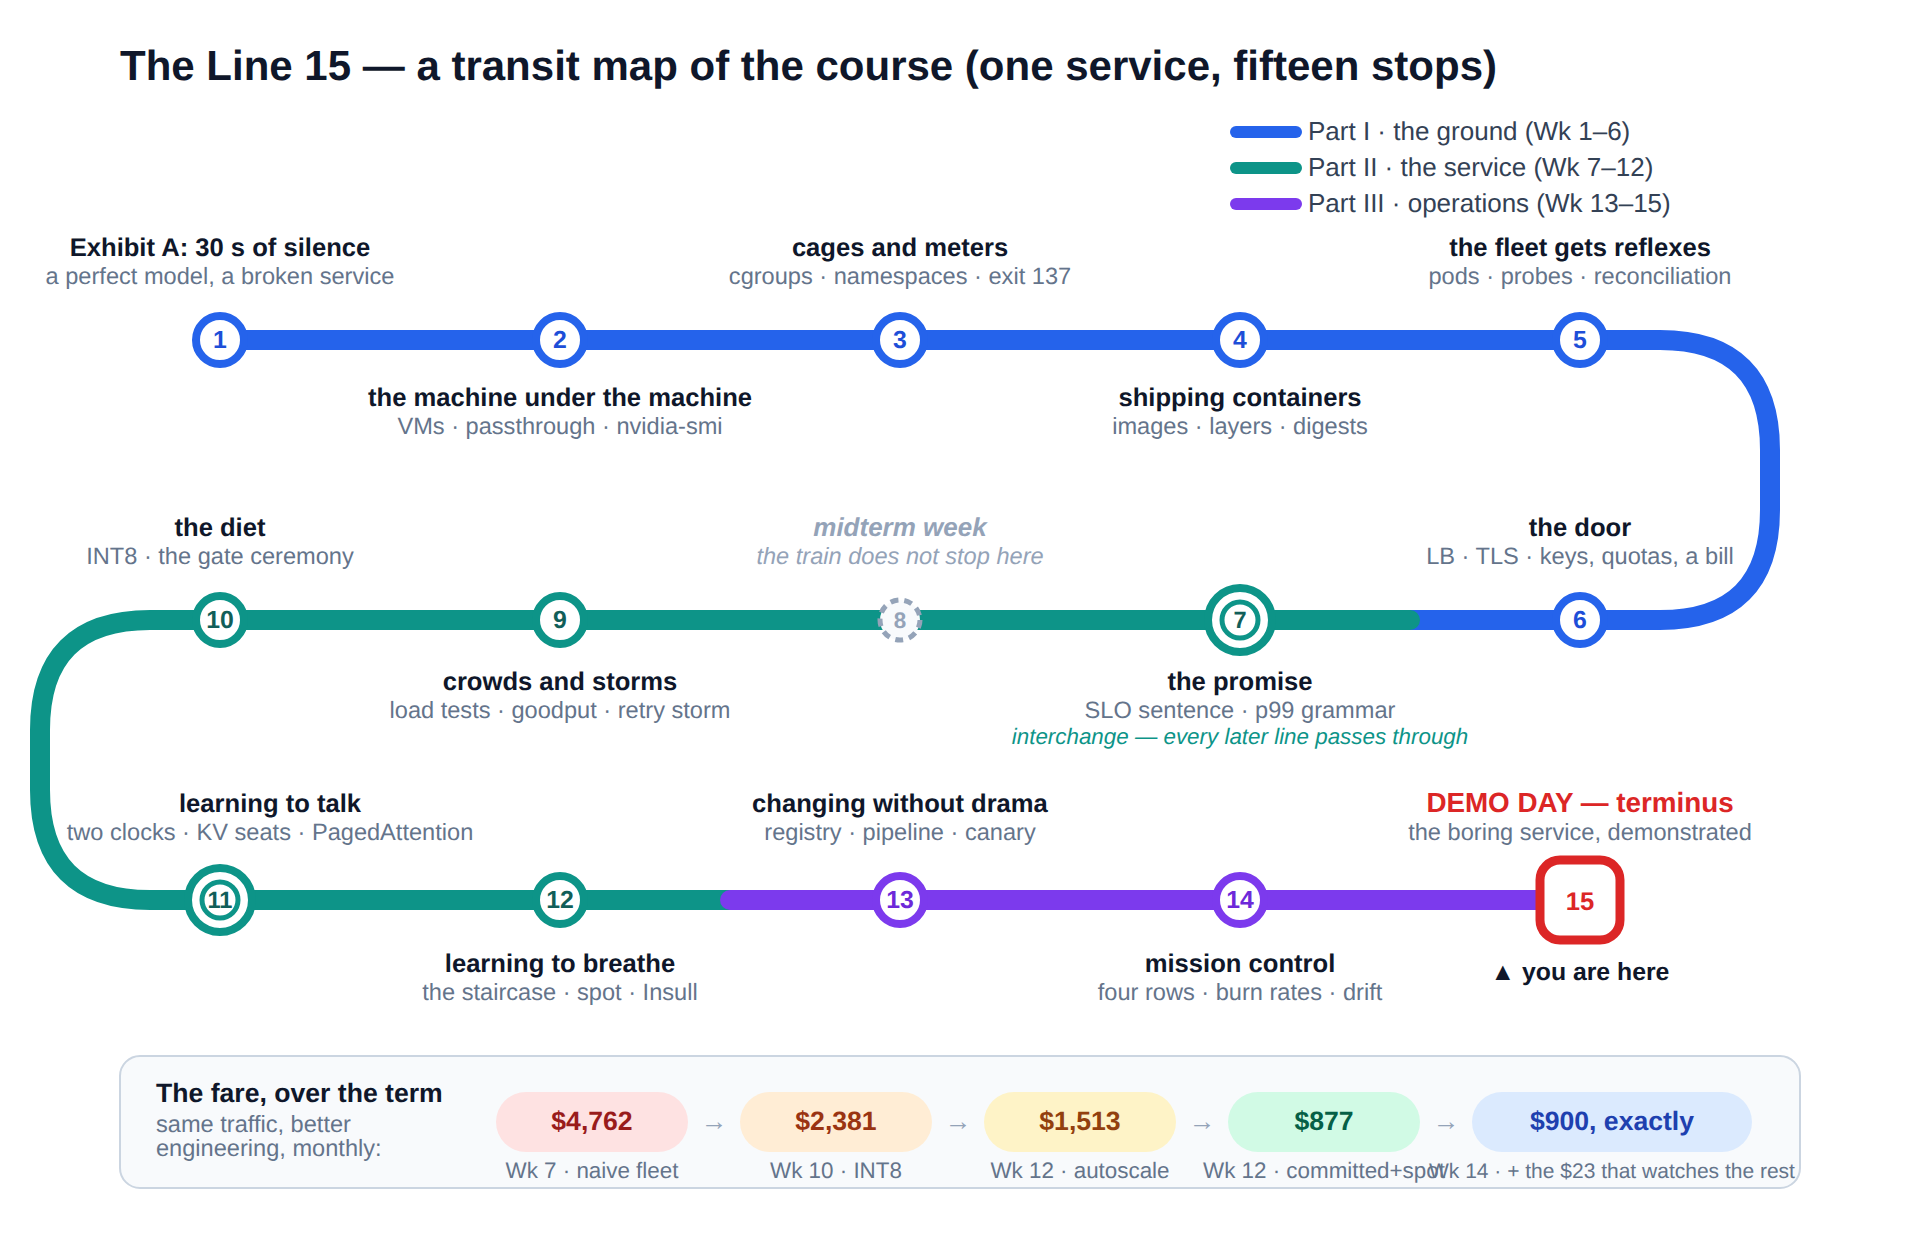
\includegraphics{figures/figE-1_line15.png}}\\[3pt]
  \figcaption{그림 E-1  15호선. 하나의 서비스, 15개 정거장, 세 개의 운임 구간. 엔지니어링이 개선될수록 운임은 4,762달러에서 스스로 선택한 900달러까지 내려간다. 열차는 8주 차에 정차하지 않는다. 종착역은 시연을 마친 지루한 서비스다. 현재 위치는 여기다.}
\end{tbbfigure}

\namedsection{E.2}{기념품 진열장}

이 책의 각 장에는 일부러 들고 다닐 수 있게 만든 문장을 적어도 하나씩 심었다. 지친 머릿속에서도 살아남을 만큼 짧고, 결정을 내릴 수 있을 만큼 날카로운 문장이다. 이는 문체상의 버릇이 아니라 핵심 설계였다. 프로덕션 엔지니어링은 대개 사람이 가장 온전하게 생각하기 어려울 때 수행한다. 새벽 2시, 데모 당일, 분기 9주 차 같은 때다. 좋은 격언은 \textbf{성능이 떨어진 하드웨어를 위한 압축}이다. 전체 논증을 미리 계산해 잠이 부족한 사람도 닿을 수 있는 곳에 캐시해 둔다. 이제 그 문장들을 얻게 된 사건과 함께 박물관 명패에 올려 두었다. 가끔 먼지를 털어 주자.

\begin{tbbtablewrap}
  \begin{tabular}{@{}>{\raggedright\arraybackslash}m{\dimexpr 0.3564\tbltextwidth-2\tabcolsep\relax} >{\raggedright\arraybackslash}m{\dimexpr 0.1596\tbltextwidth-2\tabcolsep\relax} >{\raggedright\arraybackslash}m{\dimexpr 0.4840\tbltextwidth-2\tabcolsep\relax}@{}}
  \arrayrulecolor{tbbnavy}\specialrule{1pt}{0pt}{0pt}
  \rowcolor{tbbtablehead}{\centering \bfseries\color{tbbnavy}기념품} & {\centering \bfseries\color{tbbnavy}얻은 때} & {\centering \bfseries\color{tbbnavy}오래 남는 이유} \\
  \arrayrulecolor{tbbnavy}\specialrule{0.7pt}{0pt}{2pt}
  {\textbf{exit 137: 커널의 작별 인사}} & {3주 차} & {어떤 오케스트레이터에서든 앞으로 만나게 될 모든 OOM을 설명한다. 128 + 9. 상한은 실제였고 계량기는 정직했다.} \\
  \arrayrulecolor{tbbtableborder}\hline
  {\textbf{시스템을 보는 시야는 마운트만큼 정직하다}} & {3주 차} & {네임스페이스 안의 ps부터 cgroup 파일을 읽는 익스포터까지, 무엇을 읽는지 확인하지 않으면 계측도 거짓말한다.} \\
  \arrayrulecolor{tbbtableborder}\hline
  {\textbf{태그는 떠돌지만 다이제스트는 변하지 않는다}} & {4주 차} & {13주 차의 레지스트리 전체는 이 문장이 자란 모습이다. 레이블이 아니라 내용으로 버전을 정하면 롤백은 포인터 하나가 된다.} \\
  \arrayrulecolor{tbbtableborder}\hline
  {\textbf{프로브는 반사 작용이고, 모니터링은 기억이다}} & {5→14주 차} & {관측 가능성 없는 자가 치유는 장애를 억눌러 숨기는 일이다. 두 신경계가 모두 필요하며 서로 경쟁하지 않는다.} \\
  \arrayrulecolor{tbbtableborder}\hline
  {\textbf{하나의 상태 엔드포인트가 유일한 진실 공급원이다}} & {6주 차} & {"정상"의 정의가 둘이면 분기마다 정확히 한 번, 언제나 가장 나쁜 장애에서 서로 다른 답을 낸다.} \\
  \arrayrulecolor{tbbtableborder}\hline
  {\textbf{평균은 아무도 설명하지 못한다}} & {7주 차} & {이 책에서 가장 많이 반복한 문장이다. 현장에서 가장 많이 되풀이하는 실수를 가리키기 때문이다.} \\
  \arrayrulecolor{tbbtableborder}\hline
  {\textbf{백분위수는 더할 수도, 평균 낼 수도 없다}} & {7→14주 차} & {진지한 시스템이 히스토그램을 제공하는 이유다. avg-of-p99s는 실제가 9.08초일 때 2.76초라고 말한 적이 있다.} \\
  \arrayrulecolor{tbbtableborder}\hline
  {\textbf{L = λW}} & {7→11주 차} & {회의실까지 따라오는 유일한 공식이다. 좌석, 도착률, 대기 시간을 대기열과 KV 풀 모두에 같은 대수로 적용한다.} \\
  \arrayrulecolor{tbbtableborder}\hline
  {\textbf{빠른 거절이 느린 가능성보다 낫다(거절이 곧 제품이다)}} & {9주 차} & {일찍, 싸게 덜어 내라. 헛된 대기열을 만드는 시스템은 자신의 폭풍에 스스로 먹이를 준다.} \\
  \arrayrulecolor{tbbtableborder}\hline
  {\textbf{허용 오차는 측정값보다 먼저 정한다}} & {10주 차} & {측정하기 전에 "충분히 좋다"의 뜻을 정하지 않으면 측정값이 대신 정한다. 손실 최적화에는 절차가 필요하다.} \\
  \arrayrulecolor{tbbtableborder}\hline
  {\textbf{높은 캐시 점유는 정상이고, 경보해야 할 것은 대기열이다}} & {11주 차} & {가득 찬 캐시는 설계가 작동하는 모습이다. 커지는 대기열은 수요가 좌석을 앞지른다는 뜻이다. 이 계기를 잘못 읽는 통과 의례는 건너뛰자.} \\
  \arrayrulecolor{tbbtableborder}\hline
  {\textbf{파드는 파도를 쫓고, 노드는 예보를 따른다}} & {12주 차} & {두 시간 척도, 두 메커니즘, 하나의 청구서. 여섯 단어로 요약한 오토스케일링이다.} \\
  \arrayrulecolor{tbbtableborder}\hline
  {\textbf{지루함 = 자동화 + 버전 관리 + 점진성 + 가역성(+ 관측)}} & {13→14주 차} & {14주 차의 보완을 더한 배포 문장이다. 지루하다는 말은 운영이 줄 수 있는 최고의 찬사다.} \\
  \arrayrulecolor{tbbtableborder}\hline
  {\textbf{카나리는 절벽을 잡지만 비탈은 잡지 못한다}} & {13주 차} & {모든 계측기에는 보지 못하는 시간 척도가 있다. 분 단위 계측기와 주 단위 계측기를 짝짓지 않으면 세상은 둘 사이로 흘러 지나간다.} \\
  \arrayrulecolor{tbbtableborder}\hline
  {\textbf{증상에는 호출, 원인에는 티켓}} & {14주 차} & {당직 순환을 온전하게 유지하고 호출기를 믿게 만드는 짧은 라우팅 규칙이다. 이 교훈의 수업료는 병원이 치렀다.} \\
  \arrayrulecolor{tbbtableborder}\hline
  {\textbf{새벽 2시에는 오후 2시에 그린 그래프만 보인다}} & {14주 차} & {이 책 후반부의 운영 내용을 한 문장으로 요약한다. 밤이 질문하기 전에 그 질문을 그래프로 그려 두어라.} \\
  \arrayrulecolor{tbbnavy}\specialrule{1pt}{2pt}{0pt}
  \end{tabular}\par
  \figcaption{기념품 진열장. 15주 동안 모은 16개의 명패다. 하나만 간직한다면 마지막 문장을 고르자. 나머지를 간직하는 방법까지 그 안에 들어 있다.}
\end{tbbtablewrap}

\namedsection{E.3}{저녁 만찬}

이 책에는 불안할 때 드러나는 버릇이 하나 있었다. 문제가 정말 어려워지기만 하면 방을 나섰다. 다음 장으로 간 것이 아니라 다른 \textit{세기}로 도망쳤다. 7주 차에 청구서가 도착하자 \textbf{1902년}으로 달려가 전차와 제빙 공장에 킬로와트시를 팔던 사람을 만났다. 플릿의 규모를 정해야 하자 \textbf{1961년}으로 가서 아무 가정도 하지 않았기에 어떤 상황에서도 살아남은 대기열 증명을 찾았다. KV 풀이 쓸 수 없는 조각으로 산산이 흩어지자 \textbf{1962년}의 페이지 테이블로 향했다. 배포를 판정해야 할 때는 \textbf{1890년대}로 가서 온혈의 보초를 탄광에 데려간 생리학자를 만났다. 호출기에 예절이 필요하자 \textbf{1969년} 휴스턴의 한 방으로 가서 손으로 쓴 종이에 적힌 네 자리 경보 코드를 읽었다. 이는 결코 장식이 아니었다. 눈치채지 못할 만큼 반복해서 전한 이 강의의 가장 깊은 주장이었다. \textbf{서빙의 어려운 문제는 새로운 문제가 아니다.} 단위만 바뀐 오래된 문제다. 킬로와트는 GPU 시간으로, 간선 회선은 좌석으로, 일산화탄소는 나쁜 백분위수로 바뀌었다. 먼저 그 문제를 해결한 사람들은 이제 직업적으로 여러분의 동료다.

그래서 저녁 만찬을 연다. 이 맺음말의 유일한 시험이며 스스로 치르는 시험이다. 지금의 기술 스택이 발명되기도 전에 세상을 떠난 사람들과 한 식탁에 앉아 자기 자리를 지킬 수 있는가? 15주 전의 정직한 답은 아니었다. 지능이 부족해서가 아니라 \textit{같은 청구서}를 받아 본 적이 없었기 때문이다. 유휴 용량에 돈을 내거나, 백분위수에 서명하거나, 보초 하나를 믿고 플릿을 걸거나, 깨워야 할 이유가 충분한 머신에게 잠을 깨워진 적이 없었다. 이제는 모두 경험했다. 이 사람들의 학문을 배웠기 때문이 아니라 같은 우주에서 청구서를 받았기 때문에 이 식탁에 앉을 자격이 있다. 피크와 골짜기, 좌석과 기다림, 절벽과 비탈, 작업자와 새가 적힌 같은 청구서다. 좌석도 그에 맞춰 배치했다. 각 의자의 번호는 \textbf{초대장을 보낸 주 차}다.

\begin{tbbtablewrap}
  \begin{tabular}{@{}>{\raggedright\arraybackslash}m{\dimexpr 0.0957\tbltextwidth-2\tabcolsep\relax} >{\raggedright\arraybackslash}m{\dimexpr 0.2074\tbltextwidth-2\tabcolsep\relax} >{\raggedright\arraybackslash}m{\dimexpr 0.3138\tbltextwidth-2\tabcolsep\relax} >{\raggedright\arraybackslash}m{\dimexpr 0.3830\tbltextwidth-2\tabcolsep\relax}@{}}
  \arrayrulecolor{tbbnavy}\specialrule{1pt}{0pt}{0pt}
  \rowcolor{tbbtablehead}{\centering \bfseries\color{tbbnavy}좌석} & {\centering \bfseries\color{tbbnavy}손님} & {\centering \bfseries\color{tbbnavy}같은 문제의 옛 모습} & {\centering \bfseries\color{tbbnavy}식탁에서 나눌 이야기} \\
  \arrayrulecolor{tbbnavy}\specialrule{0.7pt}{0pt}{2pt}
  {\centering \textcolor{tbbteal}{\textbf{7}}} & {\textbf{존 리틀}\newline \textit{대기행렬, 1961}} & {고객이 얼마나 빨리 도착하고 얼마나 오래 머무는지 알 때 가게 \textit{안}에 몇 명이 있는가. 두 값에 아무런 가정도 두지 않고 증명했다.} & {냅킨에 KV 풀을 그려 보이면 곧바로 알아볼 것이다. 좌석, 도착, 기다림이다. 그의 대수는 7주 차 레플리카와 11주 차 캐시에 두 번 사용했다. 그는 둘이 같은 용법이었다고 조용히 짚어 줄 것이다.} \\
  \arrayrulecolor{tbbtableborder}\hline
  {\centering \textcolor{tbbteal}{\textbf{9}}} & {\textbf{마거릿 해밀턴}\newline \textit{아폴로 소프트웨어, 1969}} & {하강 중 과부하가 걸리자 설계대로 우선순위가 낮은 작업을 버리고도 착륙에 성공한 4KB 실행 시스템.} & {군중이 몰릴 때 서비스가 무엇을 버리는지, 그 대상을 미리 정했는지 물을 것이다. 9주 차의 답을 준비하자. \textit{거절이 곧 제품이다.} 그의 소프트웨어는 달까지 날아갔고, 여러분의 서비스는 429를 반환한다. 원리는 같고 고도만 다르다.} \\
  \arrayrulecolor{tbbtableborder}\hline
  {\centering \textcolor{tbbteal}{\textbf{11}}} & {\textbf{Atlas 페이징 팀}\newline \textit{맨체스터, 1962}} & {프로그램은 연속된 메모리를 요구했지만 머신에는 흩어진 조각만 남았다. 고정 크기 페이지와 주소를 변환하는 테이블로 해결했다.} & {그들의 기술이 이제 \textit{어텐션 내부에서} 실행된다고 알려 주자. 16토큰 블록, 4\% 미만의 낭비, 2\textasciitilde{}4배의 처리량이다. 누구도 그 생각을 개선하지 않았고 목표만 바꾸어 적용했다. 놀라지 않을 것이다. 간접 참조에 익숙한 사람은 좀처럼 놀라지 않는다.} \\
  \arrayrulecolor{tbbtableborder}\hline
  {\centering \textcolor{tbbteal}{\textbf{12}}} & {\textbf{새뮤얼 인설}\newline \textit{시카고 에디슨, 1902}} & {저녁 조명 피크에 맞춰 지은 발전소는 하루 20시간 놀았다. 그의 집착은 \textbf{부하율}, 즉 피크 대비 평균 수요였다.} & {수프가 나오기도 전에 새벽 4시 GPU가 무엇을 하는지 물을 것이다. \textit{드리프트 평가가 유휴 골짜기에 올라탄다}고 답할 수 있다면, 12주 차의 약정 바닥 위에서 14주 차의 판정 작업이 돈다는 뜻이다. 디저트가 나오기 전에 채용하려 들 것이다.} \\
  \arrayrulecolor{tbbtableborder}\hline
  {\centering \textcolor{tbbpurple}{\textbf{13}}} & {\textbf{존 스콧 홀데인}\newline \textit{광산 생리학, 1896}} & {대사 속도가 더 빠른 보초를 작업자보다 먼저 노출했다. 관찰 비용과 대응 비용이 싸고 몇 분의 경고 시간을 벌었다.} & {트래픽 5\% 분할을 보고 만족할 것이다. 그의 새를 은퇴시킨 탐지기가 나오기까지 90년이 걸렸지만, 여러분의 것은 자동으로 지켜보다 몇 초 만에 후퇴한다고 담담히 말할 것이다. 그러고는 몸을 기울여 묻는다. \textit{카나리는 절벽을 잡는다. 비탈은 무엇이 지켜보는가?}} \\
  \arrayrulecolor{tbbtableborder}\hline
  {\centering \textcolor{tbbpurple}{\textbf{14}}} & {\textbf{존 에런과 잭 가먼}\newline \textit{미션 컨트롤, 1969}} & {훈련에서 본 이상한 텔레메트리 패턴 하나를 기억해 낸 SCE to AUX, \textit{실패한} 시뮬레이션 뒤 손으로 쓴 참고표로 해결한 1202.} & {새벽 2시에는 타고난 천재성보다 알아볼 수 있는 패턴이 낫다는 사실을 보여 준 최고의 두 사례다. 참고표가 어디에 있는지(런북), 어떤 실패가 그것을 쓰게 했는지(일부러 두 번 망가뜨린 실습), 장애 뒤 누가 갱신하는지 물을 것이다. 정직하게 답하자. 두 사람은 거짓말을 알아챈다.} \\
  \arrayrulecolor{tbbtableborder}\hline
  {\centering \textcolor{tbbred}{\textbf{15}}} & {\textbf{여러분}\newline \textit{15주, 하나의 서비스}} & {30초의 침묵 뒤에 있던 완벽한 모델을 약속이 글로 적힌 지루한 서비스로 바꾸었다.} & {대부분은 듣기만 하자. 청구서가 오면 비용이 부하율에 따라 나뉘고, 여러분의 금액은 스스로 고른 숫자, 곧 \textbf{정확히 900달러}로 끝난다고 말하자. 이 식탁의 모든 사람은 그 사실이 왜 그토록 만족스러운지 정확히 이해한다.} \\
  \arrayrulecolor{tbbnavy}\specialrule{1pt}{2pt}{0pt}
  \end{tabular}\par
  \figcaption{좌석 순서대로 적은 손님 명단. 1주 차부터 6주 차를 대표해 커널도 초대했지만 참석하지 못한다는 답을 보내왔다. 누군가는 불을 계속 켜 두어야 한다.}
\end{tbbtablewrap}

\begin{tbbfigure}
  \adjustbox{max width=0.94\linewidth,max totalheight=0.46\textheight}{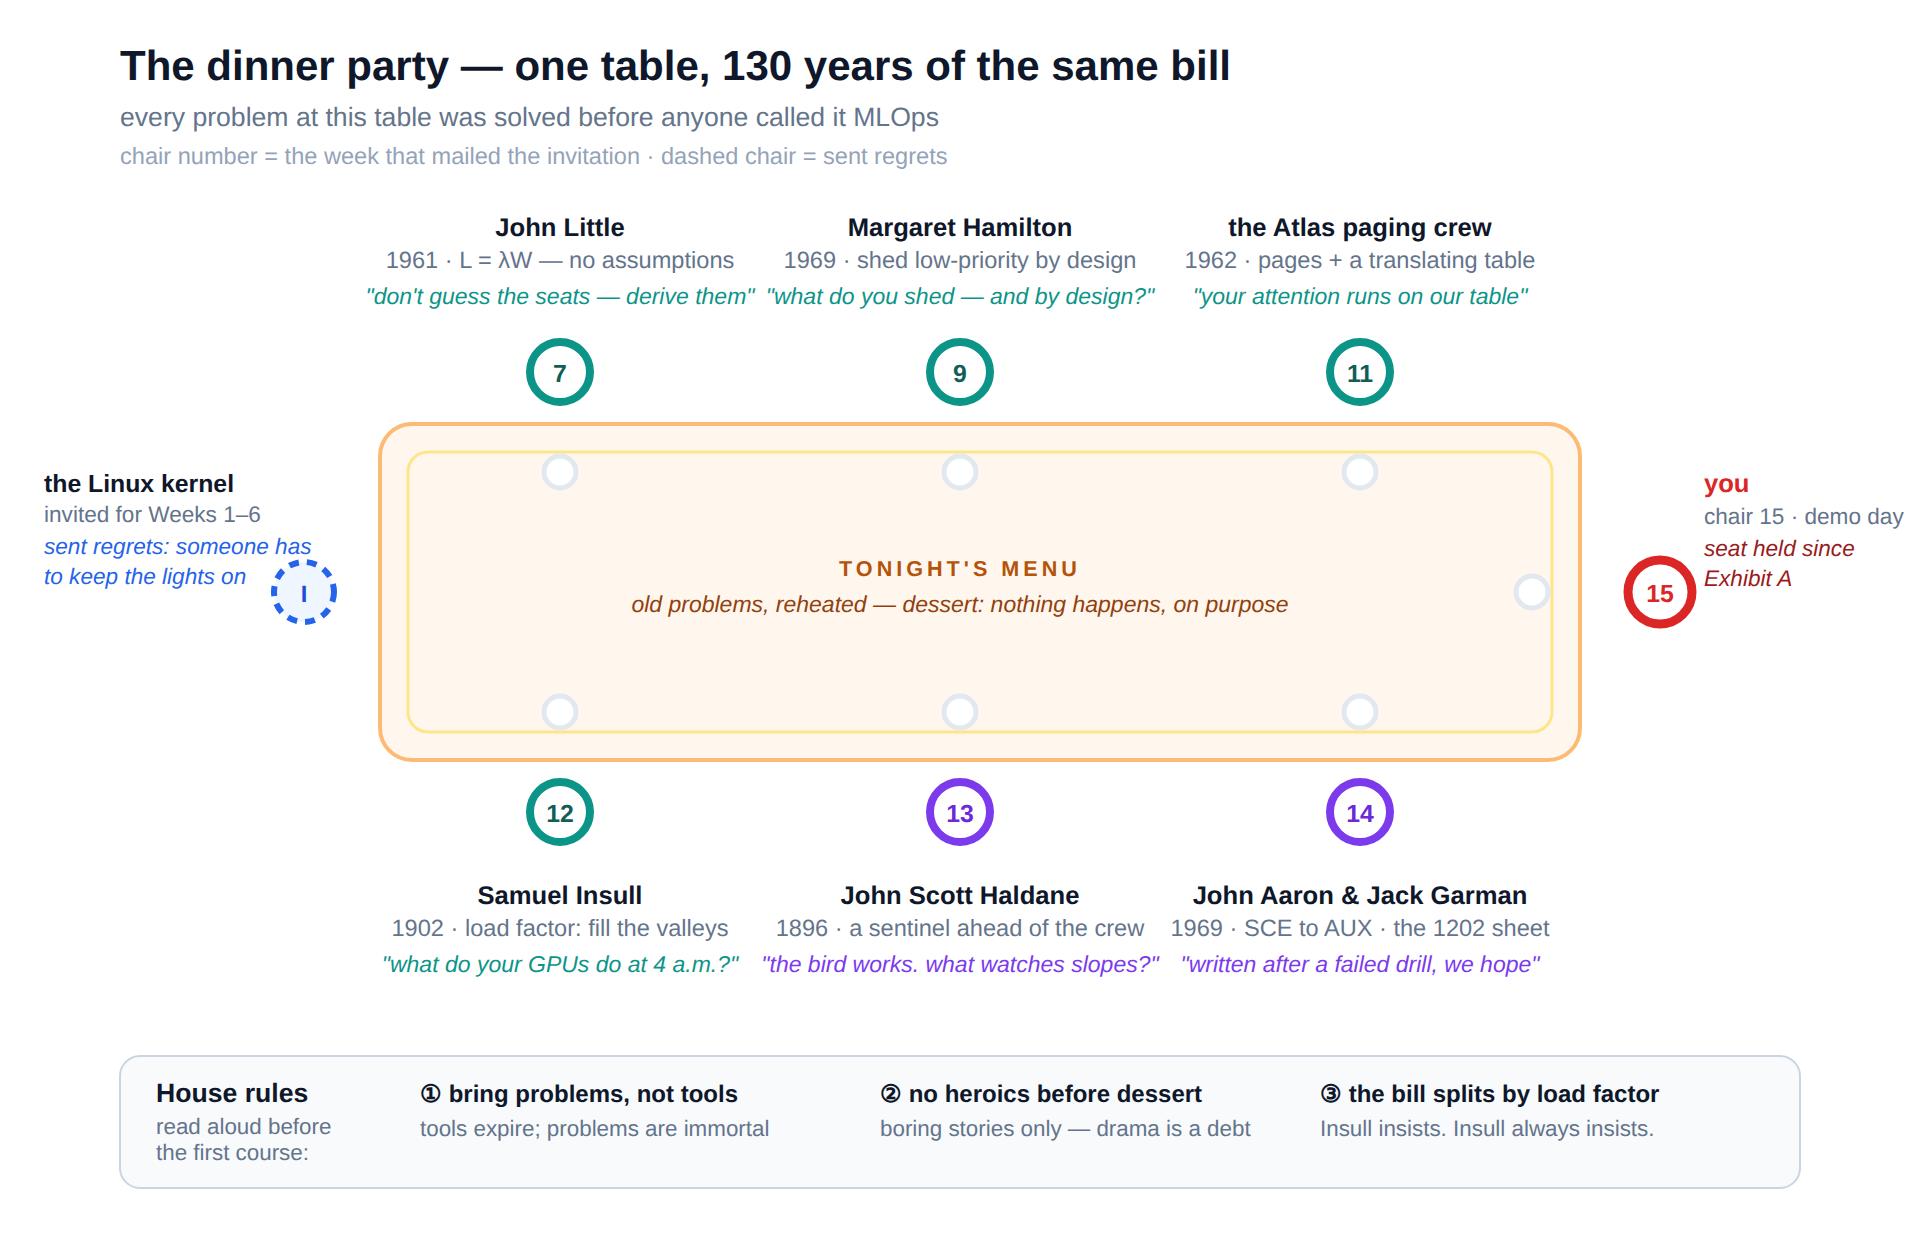
\includegraphics{figures/figE-2_dinner.png}}\\[3pt]
  \figcaption{그림 E-2  좌석 배치도. 의자 번호는 초대장을 보낸 주 차다. 커널은 불참을 알렸고, 상석은 사례 1-A 때부터 줄곧 여러분의 자리였다. 비용은 세 번째 식사 규칙에 따라 나눈다.}
\end{tbbfigure}

\begin{calloutbox}{tbbteal}{tbbtealfill}
{\normalsize\bfseries\color{tbbteal}이 만찬을 여는 까닭}\par\vspace{3pt}
이 만찬은 보상이 아니라 방법이다. 에너지든, 토큰이든, 에이전트든, 2030년대가 무엇에 계량기를 달든 다음번의 터무니없는 청구서 역시 새로운 문제는 아닐 것이다. 그 방에서 가장 빠른 엔지니어는 누구보다 먼저 이렇게 묻는 사람이다. \textit{컴퓨팅이 생기기 전에 누가 같은 청구서를 냈으며, 무엇을 측정했는가?} 더 오래된 것에서 훔쳐라. 이 식탁에는 10년에 한 번쯤 의자가 하나씩 늘어나지만 집안의 격식은 변하지 않는다. 문제만 들여보낸다. 도구는 문 앞에 맡기며, 바로 그곳에서 유효기간이 끝난다.
\end{calloutbox}

\vspace{4.0pt}

\namedsection{E.4}{보증서}

모든 기술서는 유효기간과 함께 출고되지만, 그 날짜를 인쇄한 책은 거의 없다. 독자는 면접에서 폐기된 플래그를 말하고, 사라진 가격표로 예산을 잡고, 이름이 바뀐 YAML 키 하나에 오후를 통째로 쓰면서 어렵게 사실을 깨닫는다. 그러고는 책 전체가 상했다고 잘못 결론 내린다. 그렇지 않다. 시스템 책은 혼합 화물이다. 어떤 내용은 \textbf{우유}이고, 어떤 내용은 \textbf{통조림}이며, 또 어떤 내용은 \textbf{무쇠}다. 정직한 방법은 상자마다 표지를 붙이는 것이다. 여기 눈에 보이는 잉크로 인쇄한 보증서가 있다.

유효기간을 판별하는 데는 1초면 충분하며, 이 책은 물론 어떤 책의 문장에도 적용할 수 있다. 문장에 \textit{제품명, 가격, 버전, 순위}가 들어 있는가? 우유다. 특정 실습실, 지역, 연도 안에서만 참이다. 신선할 때 소비하고 다시 인용하기 전에는 재측정해야 한다. \textit{인터페이스나 메커니즘}, 예를 들어 다이제스트, cgroup 파일, 조정 루프, 히스토그램을 말하는가? 통조림이다. 인터페이스는 조약이고 조약을 깨는 데는 큰 비용이 들기 때문에 약 10년 동안 유행의 변화를 막아 낸다. \textit{항등식, 비율, 스트레스 상황의 인간에 관한 사실}을 말하는가? 무쇠다. L = λW는 1961년에도 특혜를 요구하지 않았고 지금도 그렇다. 부하율은 진공관보다 오래되었으며 경보 피로에는 실제 희생자가 있다. 무쇠 등급은 산업 자체가 바뀌어도 살아남는다. 의미 있는 내구성 시험은 오직 이것뿐이다.

\begin{tbbtablewrap}
  \begin{tabular}{@{}>{\raggedright\arraybackslash}m{\dimexpr 0.3191\tbltextwidth-2\tabcolsep\relax} >{\raggedright\arraybackslash}m{\dimexpr 0.1596\tbltextwidth-2\tabcolsep\relax} >{\raggedright\arraybackslash}m{\dimexpr 0.5213\tbltextwidth-2\tabcolsep\relax}@{}}
  \arrayrulecolor{tbbnavy}\specialrule{1pt}{0pt}{0pt}
  \rowcolor{tbbtablehead}{\centering \bfseries\color{tbbnavy}보증 대상} & {\centering \bfseries\color{tbbnavy}등급} & {\centering \bfseries\color{tbbnavy}보증 조건} \\
  \arrayrulecolor{tbbnavy}\specialrule{0.7pt}{0pt}{2pt}
  \cellcolor{tbbxFFF7ED}{이름, 가격, 플래그: vLLM 스위치, KEDA 스케일러, GPU 시간당 비용, 4,762→900달러 장부, T4와 H100, "소형 = 1\textasciitilde{}3B", 이번 철의 양자화 방법} & \cellcolor{tbbxFFF7ED}{\centering \textcolor{tbbamberdark}{\textbf{우유}\newline \textit{90일\textasciitilde{}3년}}} & \cellcolor{tbbxFFF7ED}{숫자는 특정 실습실, 지역, 연도에서 참이었다. 실제로 얻은 것은 그 숫자를 만든 \textit{방법}, 곧 측정하고, 관문을 적용하고, 다시 측정하는 절차다. 다시 실행해 자신의 숫자를 얻자. 어차피 더 좋아져 있을 것이다.} \\
  \arrayrulecolor{tbbtableborder}\hline
  \cellcolor{tbbxFFF7ED}{순위표: Triton 대 TorchServe 대 BentoML 대 Ray Serve, SageMaker와 Vertex가 관리해 주는 것과 그렇지 않은 것} & \cellcolor{tbbxFFF7ED}{\centering \textcolor{tbbamberdark}{\textbf{우유}\newline \textit{90일\textasciitilde{}3년}}} & \cellcolor{tbbxFFF7ED}{비교표는 상하지만 \textit{머리글에 적힌 질문}은 상하지 않는다. 다음에 나오는 제품에도 같은 질문을 던지고, 승자가 달라져도 미련 없이 받아들이자.} \\
  \arrayrulecolor{tbbtableborder}\hline
  \cellcolor{tbbxEFF6FF}{인터페이스: OCI 이미지와 다이제스트, cgroup v2 파일, 조정 루프, Prometheus의 시계열 모델, HTTP 스트림} & \cellcolor{tbbxEFF6FF}{\centering \textcolor{tbbnavy}{\textbf{통조림}\newline \textit{약 10년}}} & \cellcolor{tbbxEFF6FF}{유행이 아니라 조약이다. 그 위의 대시보드는 해마다 새로 칠하지만, 아래에서는 다이제스트가 여전히 해시이고, 상한은 여전히 커널이 읽는 파일이며, 원하는 상태는 계속 수렴한다. 한 번 배워 직장을 옮겨도 가져갈 수 있다.} \\
  \arrayrulecolor{tbbtableborder}\hline
  \cellcolor{tbbxEFF6FF}{메커니즘: 연속 배칭, 페이지드 KV, 레지스트리→관문→카나리, 두 시간 척도의 오토스케일링, 플릿 백분위수용 히스토그램} & \cellcolor{tbbxEFF6FF}{\centering \textcolor{tbbnavy}{\textbf{통조림}\newline \textit{약 10년}}} & \cellcolor{tbbxEFF6FF}{가중치 스트림과 메모리 벽이라는 물리 법칙, 밤낮에 따라 움직이는 사람 때문에 존재한다. 어느 쪽에도 지원 종료 일정은 없다. 이름은 자주 바뀌고 인수되겠지만 형태는 유지된다.} \\
  \arrayrulecolor{tbbtableborder}\hline
  \cellcolor{tbbxF0FDFA}{계산: L = λW, 백분위수는 더할 수도 평균 낼 수도 없음, 평균은 아무도 설명하지 못함, 128 + 9 = 137, 부하율 = 평균 ÷ 피크} & \cellcolor{tbbxF0FDFA}{\centering \textcolor{tbbteal}{\textbf{무쇠}\newline \textit{서면 보증 10년}}} & \cellcolor{tbbxF0FDFA}{리틀은 아무 가정 없이 법칙을 증명했으므로 시간이 깨뜨릴 것이 없다. 인설의 비율은 진공관보다 오래되었다. POSIX가 137을 약속한 기간은 웹의 역사보다 길다.} \\
  \arrayrulecolor{tbbtableborder}\hline
  \cellcolor{tbbxF0FDFA}{절차: 허용 오차는 측정값보다 먼저 정함, 증상에는 호출하고 원인에는 티켓 발행, 비난 없는 사후 분석, 지루함 = 자동화 + 버전 관리 + 점진성 + 가역성(+ 관측)} & \cellcolor{tbbxF0FDFA}{\centering \textcolor{tbbteal}{\textbf{무쇠}\newline \textit{서면 보증 10년}}} & \cellcolor{tbbxF0FDFA}{스트레스 상황의 인간을 다루는 절차이며 인간에게는 업데이트가 배포되지 않는다. 병원 데이터에는 실제 희생자가 있고, 참고표에는 달 착륙이 있다. 새벽 2시가 존재하는 한 유효하다.} \\
  \arrayrulecolor{tbbtableborder}\hline
  \cellcolor{tbbxF0FDFA}{\textbf{법칙: 새벽 2시에는 오후 2시에 그린 그래프만 보인다}} & \cellcolor{tbbxF0FDFA}{\centering \textcolor{tbbteal}{\textbf{무쇠}\newline \textit{평생}}} & \cellcolor{tbbxF0FDFA}{이 법칙이 실패한다면 그 실패는 누군가 미리 그린 그래프에서만 보일 것이다. 결국 법칙이 다시 이긴 셈이다. 이 조항에 대한 보증 청구는 보통 \textit{연구 결과}라고 부른다.} \\
  \arrayrulecolor{tbbnavy}\specialrule{1pt}{2pt}{0pt}
  \end{tabular}\par
  \figcaption{보증서. 측정하지 않은 경우 무효.}
\end{tbbtablewrap}

\begin{calloutbox}{tbbamber}{tbbamberfill}
{\normalsize\bfseries\color{tbbamber}보증을 청구하는 방법}\par\vspace{3pt}
부하를 걸어 재현하고, 위 조건에 따라 대낮에 그린 그래프를 첨부한다. \textbf{상한 우유}는 결함이 아니다. 날짜를 확인하고 벤치마크를 다시 실행하되 방법은 간직하자. \textbf{10년 안에 통조림이 상했다면} 분노한 블로그 글 한 편과 업계의 진심 어린 사과를 받을 자격이 있다. \textbf{무쇠가 깨졌다면}, 예를 들어 L = λW를 이기는 대기열, 정직하게 평균 낼 수 있는 백분위수, 순수한 기억만으로 해결한 새벽 2시의 디버깅을 발견했다면 보증 문제가 아니다. 출판할 수 있는 연구 결과이며, 이 분야는 인용으로 보상한다. 지금까지 승인된 청구는 한 건도 없다.
\end{calloutbox}

\vspace{4.0pt}

\namedsection{E.5}{아직 겪지 않은 밤을 위한 편지}

이제 봉인된 물건 하나만 남았다. 제14장에서는 네 줄의 대시보드, 소진율, 같은 GPU를 쓰는 이웃, 20분, 비난 0건으로 이루어진 밤을 함께 리허설했다. 그러나 리허설은 리허설일 뿐이다. 앞으로 몇 주가 지났는지도 세지 못할 어느 날, 진짜 밤이 찾아온다. 호출기가 처음 울리고 그 반대편 서비스가 \textit{여러분의 것}인 밤이다. 실습도, 강사도, 정답지도 없다. 이 편지는 그 밤을 위한 것이다. 지금 한 번 읽어 내용을 기억해 두자. 그런 다음 미래의 자신이 비상 물품을 보관할 곳에 넣어 두자. 런북에 붙이거나, 당직 인수인계 문서에 고정하거나, 존재가 떠오르는 그 순간 읽고 있을 대시보드 뒤에 접어 두어도 좋다.

\begin{calloutbox}{tbbpurple}{tbbpurplefill}
{\normalsize\bfseries\color{tbbpurple}새벽 2시에 개봉할 것}\par\vspace{3pt}
엔지니어에게,

예정대로 이 편지를 읽고 있다면 밖은 어둡고, 무언가 잘못되었으며, 호출기가 여러분을 골랐을 것이다. 무엇이든 타이핑하기 전에 의식적으로 한 번 숨을 쉬자. 서비스는 이미 몇 분 동안 망가져 있었다. 5초쯤 더 기다릴 수 있다. 실습에서는 매주 자신의 죽음에서 살아남았다. 그만큼 죽이기 어렵도록 만든 서비스다.

이 밤은 처음이지만 이곳에는 전에 와 본 적이 있다. 지금 벌어지는 일은 전례가 없는 듯 느껴질 것이다. 이 시간의 모든 장애가 그렇다. 그러나 거의 틀림없이 다섯 명의 오랜 지인 가운데 하나다. 무언가 \textbf{가득 찼거나}(대기열, 디스크, 좌석 풀), 무언가 \textbf{종료되었거나}(종료 코드를 읽자. 137은 계량기가 정직했다는 뜻이다), 무언가 \textbf{바뀌었거나}(배포를 찾자. 설정도 변경이다. 설정은 \textit{언제나} 변경이다), 무언가 \textbf{들어왔거나}(아무것도 요청하지 않으면서 모든 것을 가져가는 실리콘 위의 이웃), 무언가 \textbf{드리프트했다}(카나리가 절벽을 지켜보는 동안 세상이 천천히 움직였다). 다섯 가족이다. 이 책에서 모두 대낮에 커피를 마시며 만나 보았다.

대시보드의 줄을 순서대로 읽자. 오후 2시의 두뇌가 아니라 바로 지금의 두뇌를 위해 그 순서로 그려 두었다. 약속부터 본다. 예산이 실제로 타고 있는가, 아니면 원인이 증상처럼 꾸미고 나타났는가? 아드레날린보다 소진율을 믿자. 둘 다 이 밤을 측정하지만 보정된 것은 하나뿐이다. 실제 장애라면 \textbf{이해하기 전에 완화하라.} 롤백은 포인터 하나를 뒤집는 일이고 맑은 정신일 때 연습해 두었다. 사용하는 것은 패배가 아니라 설계가 작동하는 모습이다. 특히 오늘 밤에는 빠른 거절이 느린 가능성보다 낫다.

진행하면서 타임스탬프를 채널에 곧바로 적자. 보기 흉하고 문장 부호가 없어도 된다. 내일의 자신은 그것을 경전처럼 읽을 것이다. 오늘 밤의 목표는 작게 유지하자. 진실이 아니라 \textit{안정}이다. 진실은 대낮에 비난 없이, 사람이 아니라 메커니즘의 이름을 적은 문서로 찾는다. 진지한 사람이라면 왜 더 일찍 보지 못했느냐고 묻지 않는다. 사후 분석은 그저 미리 보았을 패널 하나를 추가한다. 모든 화재는 연기 감지기를 남긴다. 그러면 다음 엔지니어의 밤은 20분 짧아진다. 손으로 쓴 경보 코드 한 장이 달 하강을 30초 더 평온하게 만든 것과 같다. 누군가 여러분을 위해 그렇게 했다. 이제 다음 사람을 위해 그렇게 하자.

장애가 끝나면, 그리고 체감보다 일찍 끝날 것이다, 그 결말의 모습을 눈여겨보자. 승리감이 넘치지 않는다. \textbf{지루하다.} 그래프는 가라앉고, 호출기는 어깨를 으쓱하며, 대시보드는 다시 숨을 쉰다. 김빠지는 결말이 아니라 그것이 바로 제품이다. 15주 동안 만든 것은 절대 망가지지 않는 서비스가 아니다. 누구도 그런 서비스를 만든 적은 없다. 대신 일찍 끝나는 밤, 의미가 있었던 호출, 포인터 한 번으로 적용한 수정, 조정된 경보 임계값 하나만 희생된 아침을 만들었다.

다시 잠자리에 들자. 서비스는 괜찮다. 여러분이 지루하게 만들었다. 처음 30초의 침묵에서 시작했을 때부터 바로 그것이 전부였다.

{\raggedleft \textcolor{tbbgray}{\textit{오후 2시, 불을 켜고 씀}}\par}
\end{calloutbox}

\vspace{4.0pt}

이것이 마지막 사례다. 15주 전에는 완벽한 모델이 30초의 침묵 뒤에 있었고, 방 안의 누구도 그 이유를 설명하지 못했다. 언젠가 찾아올 오늘 밤에는 지루한 서비스가 대시보드 위에서 숨을 쉬며 밀리초로 적은 약속과 스스로 선택한 숫자로 끝나는 예산을 지킨다. 아무도 지켜보지 않는다. 그럴 필요가 없기 때문이다. 이 두 문장 사이에 이 책이 하고 싶었던 모든 이야기가 놓여 있다. 15호선을 타고 종점까지 함께해 주어 고맙다.

\begin{center}
{\large \textcolor{tbbink}{\textbf{이제 지루한 무언가를 만들어 보자.}}}
\end{center}

\begin{center}
\textcolor{tbbgray}{∎}
\end{center}
